\documentclass{article}\usepackage[]{graphicx}\usepackage[]{color}
%% maxwidth is the original width if it is less than linewidth
%% otherwise use linewidth (to make sure the graphics do not exceed the margin)
\makeatletter
\def\maxwidth{ %
  \ifdim\Gin@nat@width>\linewidth
    \linewidth
  \else
    \Gin@nat@width
  \fi
}
\makeatother

\definecolor{fgcolor}{rgb}{0.345, 0.345, 0.345}
\newcommand{\hlnum}[1]{\textcolor[rgb]{0.686,0.059,0.569}{#1}}%
\newcommand{\hlstr}[1]{\textcolor[rgb]{0.192,0.494,0.8}{#1}}%
\newcommand{\hlcom}[1]{\textcolor[rgb]{0.678,0.584,0.686}{\textit{#1}}}%
\newcommand{\hlopt}[1]{\textcolor[rgb]{0,0,0}{#1}}%
\newcommand{\hlstd}[1]{\textcolor[rgb]{0.345,0.345,0.345}{#1}}%
\newcommand{\hlkwa}[1]{\textcolor[rgb]{0.161,0.373,0.58}{\textbf{#1}}}%
\newcommand{\hlkwb}[1]{\textcolor[rgb]{0.69,0.353,0.396}{#1}}%
\newcommand{\hlkwc}[1]{\textcolor[rgb]{0.333,0.667,0.333}{#1}}%
\newcommand{\hlkwd}[1]{\textcolor[rgb]{0.737,0.353,0.396}{\textbf{#1}}}%
\let\hlipl\hlkwb

\usepackage{framed}
\makeatletter
\newenvironment{kframe}{%
 \def\at@end@of@kframe{}%
 \ifinner\ifhmode%
  \def\at@end@of@kframe{\end{minipage}}%
  \begin{minipage}{\columnwidth}%
 \fi\fi%
 \def\FrameCommand##1{\hskip\@totalleftmargin \hskip-\fboxsep
 \colorbox{shadecolor}{##1}\hskip-\fboxsep
     % There is no \\@totalrightmargin, so:
     \hskip-\linewidth \hskip-\@totalleftmargin \hskip\columnwidth}%
 \MakeFramed {\advance\hsize-\width
   \@totalleftmargin\z@ \linewidth\hsize
   \@setminipage}}%
 {\par\unskip\endMakeFramed%
 \at@end@of@kframe}
\makeatother

\definecolor{shadecolor}{rgb}{.97, .97, .97}
\definecolor{messagecolor}{rgb}{0, 0, 0}
\definecolor{warningcolor}{rgb}{1, 0, 1}
\definecolor{errorcolor}{rgb}{1, 0, 0}
\newenvironment{knitrout}{}{} % an empty environment to be redefined in TeX

\usepackage{alltt}

% Load required packages
\usepackage{amsmath, bm, booktabs, framed, hyperref, natbib}

\hypersetup{
    colorlinks=true,
    linkcolor=blue,
    citecolor=blue,
    urlcolor=blue
}

\bibliographystyle{plainnat}

% Define macros
\newcommand{\boot}{\ensuremath{^\star}}
\newcommand{\trans}{\ensuremath{^\top}}
\newcommand{\diag}{\operatorname{diag}}
\newcommand{\col}{\operatorname{col}}
\newcommand{\row}{\operatorname{row}}
\newcommand{\COV}{\operatorname{COV}}
\newcommand{\VAR}{\operatorname{VAR}}
\newcommand{\SE}{\operatorname{SE}}
\newcommand{\E}{\operatorname{E}}
\IfFileExists{upquote.sty}{\usepackage{upquote}}{}
\begin{document}




%%%%%%%%%%%%%%%%%%%%%%%%%%%%%%%%%%%%%%%%%%%%%%%%%%%%%%%%%%%%%%%%%%%%%%%%%%%%%%%%
% Abstract
%%%%%%%%%%%%%%%%%%%%%%%%%%%%%%%%%%%%%%%%%%%%%%%%%%%%%%%%%%%%%%%%%%%%%%%%%%%%%%%%

\begin{abstract}
Keep it to 200 words or less.
\end{abstract}


%%%%%%%%%%%%%%%%%%%%%%%%%%%%%%%%%%%%%%%%%%%%%%%%%%%%%%%%%%%%%%%%%%%%%%%%%%%%%%%%
% Introduction
%%%%%%%%%%%%%%%%%%%%%%%%%%%%%%%%%%%%%%%%%%%%%%%%%%%%%%%%%%%%%%%%%%%%%%%%%%%%%%%%

\section{Introduction}

Consider an ordinary regression model $\mathcal{Y}_i = f\left(x_i; \bm{\beta} \right) + \epsilon_i$ $(i = 1, \dotsc, n)$, where $f$ is a known expectation function (called a \emph{calibration curve}) that is monotonic over the range of interest and $\epsilon_i \stackrel{iid}{\sim} \mathcal{N}\left( 0, \sigma^2 \right)$.  A common problem in regression is to predict a future response $\mathcal{Y}_0$ (or estimate the mean response $f_0$) for a known value of the explanatory variable $x_0$.  Often, however, there is a need to do the reverse; that is, given an observed value of the response $\mathcal{Y} = y_0$ (or a specified value of the mean response), estimate the unknown value of the explanatory variable $x_0$.  This is known as the \emph{calibration problem}, though we refer to it more generally as inverse estimation.  A thorough overview of the calibration problem is given in \citet{osborne-statistical-1991}.  \citet{oman-calibration-1998} considers the case of a random intercept and slope model. In this paper, we discuss inverse estimation in the more general context of linear mixed-effects models. In Section~\ref{sec:point}, we extend the classical inverse estimate. Section~\ref{sec:wald} and Sections~\ref{sec:inversion} discuss approximate interval estimates by extending the classical Wald and inversion methods, respectively. Section~\ref{sec:boot} introduces a fully parametric bootstrap algorithm for making inference on $x_0$. 


%%%%%%%%%%%%%%%%%%%%%%%%%%%%%%%%%%%%%%%%%%%%%%%%%%%%%%%%%%%%%%%%%%%%%%%%%%%%%%%%
% Linear mixed-effects models
%%%%%%%%%%%%%%%%%%%%%%%%%%%%%%%%%%%%%%%%%%%%%%%%%%%%%%%%%%%%%%%%%%%%%%%%%%%%%%%%

\section{Linear mixed-effects models}

Linear regression models with random coefficients can be represented in many different (but equivalent) forms.  One of the most common forms, attributed to \citet{laird-random-1982}, is
\begin{equation}
\label{eqn:lmm-laird-and-ware}
  \bm{\mathcal{Y}}_i = \bm{X}_i\bm{\beta} + \bm{Z}_i\bm{b}_i + \bm{\epsilon}_i, \quad i = 1, \dotsc, m,
\end{equation}
where
\begin{itemize}
  \item $\bm{\mathcal{Y}}_i$ is an $n_i \times 1$ response vector for the $i$-th subject/cluster/group;
  \item $\bm{X}_i$ is an $n_i \times p$ design matrix for the fixed effects;
  \item $\bm{Z}_i$ is an $n_i \times q$ design matrix for the random effects;
  \item $\bm{\beta}$ is a $p \times 1$ vector of fixed effects coefficients;
  \item $\bm{b}_i$ is a $q \times 1$ vector of random effects coefficients with mean zero and variance-covariance matrix $\bm{D}$;
  \item $\bm{D}$ is a $q \times q$ variance-covariance matrix for the random effects;
  \item $\bm{\epsilon}_i$ is an $n_i \times 1$ vector of random errors with mean zero and variance-covariance matrix $\sigma^2\bm{I}$.
\end{itemize}
Equation~\eqref{eqn:lmm-laird-and-ware} is known as a linear mixed-effects model (LMM).  The random effects and errors are often assumed to follow a normal distribution.  By stacking the data, the (normal) LMM can be written concisely as
\begin{equation}
\label{eqn:lmm-stacked}
    \bm{\mathcal{Y}} = \bm{X}\bm{\beta} + \bm{Z}\bm{b} + \bm{\epsilon}, \quad
      \begin{bmatrix}
        \bm{b} \\
        \bm{\epsilon}
      \end{bmatrix} \sim
      \mathcal{N}\left(\begin{bmatrix}
        \bm{0} \\
        \bm{0}
      \end{bmatrix}, \begin{bmatrix}
        \bm{D} & \bm{0} \\
        \bm{0} & \sigma^2\bm{I}
      \end{bmatrix}\right),
\end{equation}
where $\bm{\mathcal{Y}} = \col\left\{\bm{\mathcal{Y}}_i\right\}$, $\bm{X} = \col\left\{\bm{X}_i\right\}$, $\bm{Z} = \diag\left\{\bm{Z}_i\right\}$, $\bm{b} = \col\left\{\bm{b}_i\right\}$, and $\bm{\epsilon} = \col\left\{\bm{\epsilon}_i\right\}$ for $i = 1, \dotsc, m$.  Since $\COV\left[\bm{b}, \bm{\epsilon}\right] = \bm{0}$, it is assumed that the random vectors $\big\{ \bm{b}_i, \bm{\epsilon}_i \big\}_{i=1}^m$ are mutually independent.

The additional term $\bm{Z}\bm{b}$ in the model imposes a specific variance-covariance structure on the response vector $\bm{\mathcal{Y}}$:
\[
  \bm{\mathcal{Y}} \sim \mathcal{N}\left(\bm{X}\bm{\beta}, \bm{V}\right), \quad \bm{V} = \bm{Z}\bm{D}\bm{Z}\trans + \sigma^2\bm{I}.
\]
Thus, the fixed effects determine the mean of $\bm{\mathcal{Y}}$, while the random effects govern the variance-covariance structure of $\bm{\mathcal{Y}}$.  Different random effects structures impose different variance-covariance structures on the response resulting in a highly flexible framework for modelling \emph{grouped data}.

The random effects variance-covariance matrix $\bm{D}$ has at most $q(q+1)/2$ unique elements which we represent by the vector $\bm{\theta}$.  There are a number of methods available for estimating $\left( \bm{\beta}, \sigma^2, \bm{\theta} \right)$; see, for example, \citet[chap 6.]{mcculloch_generalized_2008} and \citet[chap. 2]{demidenko_mixed_2013}.  Most commonly, the fixed-effects $\bm{\beta}$ are estimated via the method of maximum likelihood (ML), while the variance components $\left(\sigma^2, \bm{\theta}\right)$ are estimated via restricted maximum likelihood (REML).  The ML estimator of $\bm{\beta}$, given by
\begin{equation*}
\widehat{\bm{\beta}} = \left( \bm{X}\trans \widehat{\bm{V}}^{-1} \bm{X} \right)\bm{X}\trans\bm{\mathcal{Y}},
\end{equation*}
depends on the estimated variance components through $\widehat{\bm{V}}$ which makes it difficult to capture the variability of $\widehat{\bm{\beta}}$ in small sample sizes (see \citet[pp. 165-167]{mcculloch_generalized_2008}).  The usual practice is to ignore the variability of the estimated variance components when making inference about the fixed effects; that is, treat $\widehat{\bm{V}}$ as the true (fixed) value of $\bm{V}$.  Modern computational procedures such as the parametric bootstrap and Markov chain Monte Carlo (MCMC) methods are two ways account for the variability of the estimated variance components.


%%%%%%%%%%%%%%%%%%%%%%%%%%%%%%%%%%%%%%%%%%%%%%%%%%%%%%%%%%%%%%%%%%%%%%%%%%%%%%%%
% Bladder volume data
%%%%%%%%%%%%%%%%%%%%%%%%%%%%%%%%%%%%%%%%%%%%%%%%%%%%%%%%%%%%%%%%%%%%%%%%%%%%%%%%

\subsection{Bladder volume data}
For illustration, let us consider the bladder volume data which can be found in \citet[pg. 7]{brown-measurement-1993} and \citet{oman-calibration-1998}.  In Brown's words:
\begin{quotation}
\noindent``A series of 23 women patients attending a urodynamic clinic were recruited for the study. After successful voiding of the bladder, sterile water was introduced in additions of 1, 1.5, and then 2.5 cl increments up to a final cumulative total of 17.5 cl. At each volume a measure of height (\texttt{H}) in mm and depth (\texttt{D}) in mm of largest ultrasound bladder images were taken. The product \texttt{H} $\times$ \texttt{D} was taken as a measure of liquid volume.''
\end{quotation}
We took Brown's suggestion and transformed the data so that the relationship is approximately linear.  Spaghettiplots of both the original and transformed data are displayed in Figure~\ref{fig:spaghetti}.

\begin{knitrout}
\definecolor{shadecolor}{rgb}{0.969, 0.969, 0.969}\color{fgcolor}\begin{figure}[!htb]
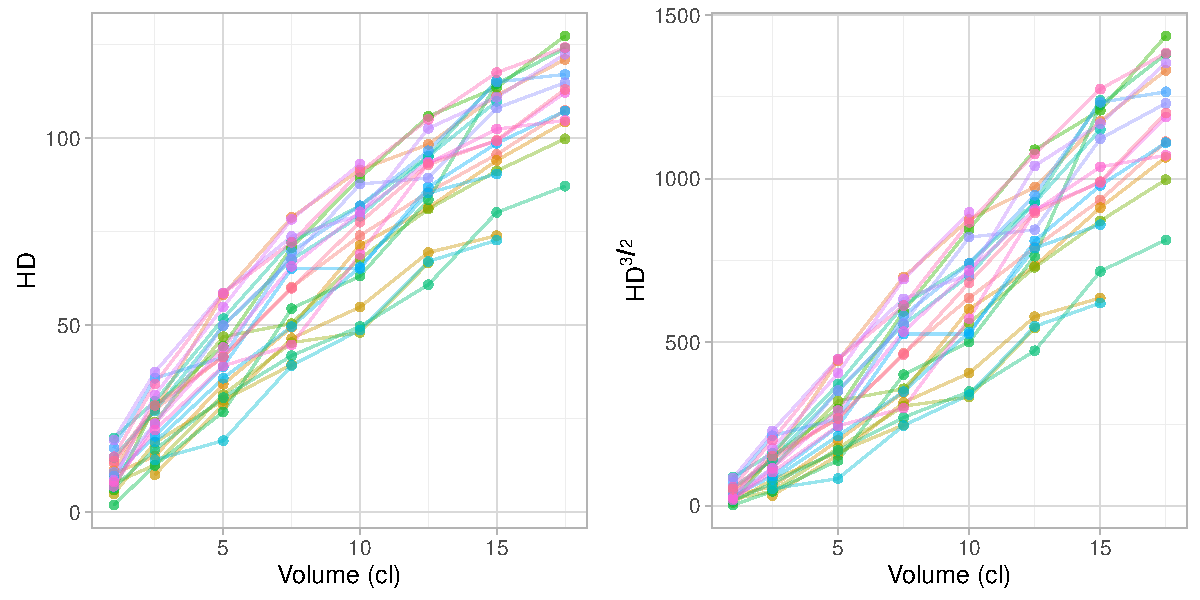
\includegraphics[width=\linewidth]{figure/spaghetti-1} \caption{Spaghettiplot of bladder volume data (lines connect measurements belonging to the same subject). \textit{Left}: Original data. \textit{Right}: Transformed data.}\label{fig:spaghetti}
\end{figure}


\end{knitrout}

A random intercept and slope model with uncorrelated random effects fits the transformed data (right side of Figure~\ref{fig:spaghetti}) well:
\begin{align*}
  \texttt{HD}^{3/2}_{ij} &= \left(\beta_0 + b_{0i}\right) + \left(\beta_1 + b_{1i}\right)\texttt{volume}_{ij} + \epsilon_{ij} \\
  b_{ki} &\sim \mathcal{N}\left(0, \theta_k^2\right), \quad k = 0, 1, \\
  \epsilon_{ij} &\sim \mathcal{N}\left(0, \sigma^2\right),
\end{align*}
where $\COV\left[b_{0i}, b_{1i}\right] = 0$.  To fit such a model in \texttt{R}, we can use the recommended \texttt{nlme} package \citep{pinheiro-nlme-2013}:
\begin{knitrout}
\definecolor{shadecolor}{rgb}{0.969, 0.969, 0.969}\color{fgcolor}\begin{kframe}
\begin{alltt}
\hlkwd{library}\hlstd{(nlme)}  \hlcom{# nlme should already be installed}
\hlstd{(fit.nlme} \hlkwb{<-} \hlkwd{lme}\hlstd{(HD}\hlopt{^}\hlstd{(}\hlnum{3}\hlopt{/}\hlnum{2}\hlstd{)} \hlopt{~} \hlstd{volume,}
                 \hlkwc{random} \hlstd{=} \hlkwd{list}\hlstd{(}\hlkwc{subject} \hlstd{=} \hlkwd{pdDiag}\hlstd{(}\hlopt{~}\hlstd{volume)),}
                 \hlkwc{data} \hlstd{= bladder,} \hlkwc{na.action} \hlstd{= na.omit))}
\end{alltt}
\begin{verbatim}
## Linear mixed-effects model fit by REML
##   Data: bladder 
##   Log-restricted-likelihood: -943
##   Fixed: HD^(3/2) ~ volume 
## (Intercept)      volume 
##       -53.8        69.1 
## 
## Random effects:
##  Formula: ~volume | subject
##  Structure: Diagonal
##         (Intercept) volume Residual
## StdDev:        39.6   14.3     53.7
## 
## Number of Observations: 166
## Number of Groups: 23
\end{verbatim}
\end{kframe}
\end{knitrout}
The \texttt{pdDiag} function forces a diagonal variance-covariance structure on the random effects; hence, a covariance of zero. The same model, but with an additional quadratic term, provides a useful fit to the original data (left side of Figure~\ref{fig:spaghetti}):
\begin{align*}
  \texttt{HD}_{ij} &= \left(\beta_0 + b_{0i}\right) + \left(\beta_1 + b_{1i}\right)\texttt{volume}_{ij} + \beta_2\texttt{volume}_{ij}^2 + \epsilon_{ij} \\
  b_{ki} &\sim \mathcal{N}\left(0, \theta_k^2\right), \quad k = 0, 1, \\
  \epsilon_{ij} &\sim \mathcal{N}\left(0, \sigma^2\right).
\end{align*}
For an in-depth treatment on fitting LMMs using the \texttt{nlme} software, see \citet{pinheiro-mixed-2000}.


%%%%%%%%%%%%%%%%%%%%%%%%%%%%%%%%%%%%%%%%%%%%%%%%%%%%%%%%%%%%%%%%%%%%%%%%%%%%%%%%
% Point estimation
%%%%%%%%%%%%%%%%%%%%%%%%%%%%%%%%%%%%%%%%%%%%%%%%%%%%%%%%%%%%%%%%%%%%%%%%%%%%%%%%

\section{Point estimation}\label{sec:point}

The standard methods of calibration, (i.e., the Wald-based and inversion confidence intervals) are easily extended to the case of random coefficients.  For convenience, let us write the linear random coefficient model as
\begin{equation*}
  \mathcal{Y}_{ij} = f\left(x_{ij}; \bm{\beta}\right) + R\left(x_{ij}; \bm{b}_i\right) + \epsilon_{ij},
\end{equation*}
where $f(\cdot)$ and $R(\cdot)$ are linear in $\bm{\beta}$ and $\bm{b}_i$, respectively.  For instance, the model for the transformed bladder data has $f\left(\texttt{volume}_{ij}; \bm{\beta}\right) = \beta_0 + \beta_1 \texttt{volume}_{ij}$ and $R\left(\texttt{volume}_{ij}; \bm{b}_i\right) = b_{0i} + b_{1i}\texttt{volume}_{ij}$ with $\E\left[R\left(\texttt{volume}_{ij}; \bm{b}_i\right)\right] = 0$ and $\VAR\left[R\left(\texttt{volume}_{ij}; \bm{b}_i\right)\right] = \theta_0^2 + \texttt{volume}_{ij}^2\theta_1^2$.

Assume that, after the data are collected and a model is fitted, we obtain a new observation, denoted $\mathcal{Y}_0$, from the same population under study for which the value of the explanatory variable $x_0$ is unknown.  We assume that the new observation belongs to a group not included in our analysis.  Estimating $x_0$ is rather straightforward.  By assumption, the new observation $\mathcal{Y}_0$ is distributed as a $\mathcal{N}\left\{f\left(x_0; \bm{\beta}\right), \sigma_0^2\right\}$ random variable with $\sigma_0^2 = \VAR\left[ R\left( x_0; \bm{b}_0 \right) \right ] + \sigma^2$.  A natural estimator for $x_0$ is then
\begin{equation}
\label{eqn:est}
  \widehat{x}_0 = f^{-1}\left(\mathcal{Y}_0; \widehat{\bm{\beta}}\right),
\end{equation}
where $\widehat{\bm{\beta}}$ is the ML estimator of $\bm{\beta}$.  We shall refer to Equation~\eqref{eqn:est} as the classical estimator.  Note that the point estimate $\widehat{x}_0$ does not involve any of the random effects; the random effects only contribute to the variance-covariance structure of the response.


%%%%%%%%%%%%%%%%%%%%%%%%%%%%%%%%%%%%%%%%%%%%%%%%%%%%%%%%%%%%%%%%%%%%%%%%%%%%%%%%
% Wald interval
%%%%%%%%%%%%%%%%%%%%%%%%%%%%%%%%%%%%%%%%%%%%%%%%%%%%%%%%%%%%%%%%%%%%%%%%%%%%%%%%

\section{Wald interval}\label{sec:wald}

An approximate $100(1-\alpha)\%$ Wald-type confidence interval for $x_0$ has the simple form
\begin{equation}
\label{eqn:wald}
  CI_{wald} = \left( \widehat{x}_0 -  \SE\left[\widehat{x}_0\right]\Phi\left(\alpha/2\right),  \widehat{x}_0 -  \SE\left[\widehat{x}_0\right]\Phi\left(1-\alpha/2\right) \right).
\end{equation}
There is no ``textbook'' formula for the standard error of $\widehat{x}_0$, instead, an estimate of this standard error is obtained using a first-order Taylor series approximation, or better yet, a bootstrap approximation.  For the Taylor series approximation, we need the variance-covariance matrix of $\left(\mathcal{Y}_0, \widehat{\bm{\beta}}\right)$,
\[
\Sigma = \begin{bmatrix}
           \VAR\left[\mathcal{Y}_0\right] & \bm{0} \\
           \bm{0} & \VAR\left[\widehat{\bm{\beta}}\right]
         \end{bmatrix} = \begin{bmatrix}
           \sigma_0^2 & \bm{0} \\
           \bm{0} & \left(\bm{X}\trans\bm{V}^{-1}\bm{X}\right)^{-1}
         \end{bmatrix}.
\]
Since $\mathcal{Y}_0$ is independent of $\bm{\mathcal{Y}}$, it is also independent of $\widehat{\bm{\beta}}$, hence the diagonal structure of $\Sigma$. Recall that our point estimate has the form $x = f^{-1}\left(y; \bm{\beta}\right)$. Let $f_1^{-1}\left(y; \bm{\beta}\right)$ and $f_2^{-1}\left(y; \bm{\beta}\right)$ denote the partial derivatives of $f^{-1}$ with respect to the parameters $y$ and $\bm{\beta}$, respectively. Our point estimator is given by $f^{-1}\left(\mathcal{Y}_0; \widehat{\bm{\beta}}\right)$, where $\mathcal{Y}_0$ is a new observation and $\widehat{\bm{\beta}}$ is the ML estimator of $\bm{\beta}$.  A first-order Taylor-series approximation for the variance of $\widehat{x}_0$ is given by
\begin{align}
  \VAR\left[\widehat{x}_0\right] &= \left[f_1^{-1}\left(\mathcal{Y}_0; \widehat{\bm{\beta}}\right)\right]^2\sigma_0^2 \nonumber \\
   &+ \left[f_2^{-1}\left(\mathcal{Y}_0; \widehat{\bm{\beta}}\right)\right]\trans\left(\bm{X}\trans\bm{V}^{-1}\bm{X}\right)^{-1}\left[f_2^{-1}\left(\mathcal{Y}_0; \widehat{\bm{\beta}}\right)\right].
\end{align}
To obtain $\SE\left[\widehat{x}_0\right] = \Big\{ \widehat{\VAR}\left[\widehat{x}_0\right] \Big\}^{1/2}$, we simply replace $\sigma_0^2$ and $\bm{V}$ with their respective estimates $\widehat{\sigma}_0^2$ and $\widehat{\bm{V}}$.

The Wald-based interval is simple to compute as long as we have an estimate for the standard error.  As we will discuss in Section~\ref{sec:implementation}, the \texttt{R} package \texttt{investr} \citep{investr-package} can be used to obtain the Wald-based interval \eqref{eqn:wald} using a Taylor series approximation of the standard error.  If a closed-form formula is available for $\widehat{x}_0$, then the \texttt{deltaMethod} function from the \texttt{car} package \citep{fox-car-2011} can also be used to obtain the Taylor series approximation of the standard error.  Alternatively, one can use a parametric bootstrap estimate of the standard error instead of relying on a Taylor series approximation --- see Section~\ref{sec:percentile}.  The bootstrap estimate may be more accurate in smaller sample sizes because, unlike the Taylor approximation estimate, it takes into account the variability of the estimated variance components.  The new \texttt{bootMer} function in the \texttt{lme4} package \citep{bates-lme4-2014} can be used for model-based parametric bootstrapping in mixed models.


%%%%%%%%%%%%%%%%%%%%%%%%%%%%%%%%%%%%%%%%%%%%%%%%%%%%%%%%%%%%%%%%%%%%%%%%%%%%%%%%
% Inversion interval
%%%%%%%%%%%%%%%%%%%%%%%%%%%%%%%%%%%%%%%%%%%%%%%%%%%%%%%%%%%%%%%%%%%%%%%%%%%%%%%%

\section{Inversion interval}\label{sec:inversion}

In the case of the simple linear regression model with constant variance, an exact $100(1-\alpha)\%$ confidence interval for $x_0$ can be derived \citep{graybill-theory-1976}.  This can be generalized to an approximate method in the case of polynomial or nonlinear regression models with independent observations and constant variance (see \citet{seber-nonlinear-2003} and \citet{huet-statistical-2004}).  In a similar fashion, we can generalize the same results to an approximate method for random coefficient models.  Let $\widehat{f}_0 = f\left(x_0; \widehat{\bm{\beta}}\right)$ be the predicted mean at $x = x_0$.  A prediction interval for $\mathcal{Y}_0$ at $x_0$ with asymptotic coverage probability $100(1-\alpha)\%$ is
\begin{equation}
\label{eqn:asymptotic-pi}
  \mathcal{I}_\infty\left(x_0\right) = \widehat{f}_0 \pm z_{1-\alpha/2}\left\{ \widehat{\VAR}\left[\mathcal{Y}_0 - \widehat{f}_0\right] \right\}^{1/2}.
\end{equation}
If instead, $\mathcal{Y}_0$ is observed to be $y_0$ and $x_0$ is unknown, then an asymptotic $100(1-\alpha)\%$ confidence interval for the unknown $x_0$ can be obtained by inverting \eqref{eqn:asymptotic-pi}:
\begin{equation}
\label{eqn:inversion}
  CI_{inv} = \left\{ x: z_{\alpha/2} \le \frac{\mathcal{Y}_0-f\left(x; \widehat{\bm{\beta}}\right)}{\left\{ \widehat{\VAR}\left[\mathcal{Y}_0 - f\left(x; \widehat{\bm{\beta}}\right)\right] \right\}^{1/2}} \le z_{1-\alpha/2} \right\}.
\end{equation}
This is known as the \emph{inversion interval} and typically cannot be written in closed-form; therefore, numerical techniques are required to find the lower and upper bounds.  Further, note that $CI_{inv}$ is not symmetric about $\widehat{x}_0$ and will not necessarily result in a single finite interval.

Fortunately, the inversion interval \eqref{eqn:inversion} can be computed automatically using the \texttt{investr} package.  However, like the Wald-based interval \eqref{eqn:wald}, the inversion interval ignores the variability of the estimated variance components and will likely perform poorly in small sample sizes.  An alternative approach involving the parametric bootstrap will be discussed in Section~\ref{sec:parboot-inversion}.

Finally, the inversion interval uses a normal approximation.  While it is likely that a $t$~distribution with some finite degrees of freedom may be more accurate, it is difficult to find the appropriate degrees of freedom. \citet{oman-calibration-1998}, suggests a $t$~distribution with $N-1$ degrees of freedom ($N$ being the total sample size).


%%%%%%%%%%%%%%%%%%%%%%%%%%%%%%%%%%%%%%%%%%%%%%%%%%%%%%%%%%%%%%%%%%%%%%%%%%%%%%%%
% Parametric bootstrap
%%%%%%%%%%%%%%%%%%%%%%%%%%%%%%%%%%%%%%%%%%%%%%%%%%%%%%%%%%%%%%%%%%%%%%%%%%%%%%%%

\section{Parametric bootstrap}\label{sec:boot}

The bootstrap \citep{efron-bootstrap-1979} is a general-purpose computer-based method for assessing accuracy of estimators and forming confidence intervals for parameters.  \citet{jones-bootstrapping-1999} proposed a nonparametric bootstrap algorithm for controlled calibration with independent observations.  However, since our application involves random coefficients (i.e., dependent observations), the nonparametric bootstrap does not easily apply, and instead, we adopt a ``fully parametric'' approach.  In a parametric bootstrap, bootstrap samples are generated from a fitted parametric model rather than sampling with replacement directly from the data.  Fortunately, parametric bootstrap confidence intervals are usually more accurate than nonparametric ones, however, by sampling from a fitted parametric family, we are implicitly assuming that we have the ``correct model''.

Let $\widehat{\sigma}_0^2$ be an estimate of the variance of the new observation $\mathcal{Y}_0$.  An algorithm for bootstrapping $\widehat{x}_0$ in an LMM is given in Figure~\ref{fig:parboot}.  Note that step 5. is crucial for calibration problems because we need to treat $y_0$ as a random quantity in the bootstrap simulation, otherwise the variability of $\widehat{x}_0$ will be underestimated; see, for example, \citet{jones-bootstrapping-1999} and \citet{greenwell-investr-2014}.
\begin{figure}[!htb]
\begin{enumerate}
  \item Fit a mixed model \eqref{eqn:lmm-stacked} to the data and obtain estimates $\widehat{\bm{\beta}}$, $\widehat{\bm{D}}$, and $\widehat{\sigma}^2$.
	\item Define $\bm{y}\boot = \bm{X}\widehat{\bm{\beta}} + \bm{Z}\bm{b}\boot + \bm{\epsilon}\boot$, where $\bm{b}\boot \sim \mathcal{N}_q\left(\bm{0}, \widehat{\bm{D}}\right)$ and $\bm{\epsilon}\boot \sim \mathcal{N}_N\left(\bm{0}, \widehat{\sigma}_\epsilon^2\bm{I}\right)$;
	\item Update the original model using $\bm{y}\boot$ as the response vector to obtain $\widehat{\bm{\beta}}\boot$ and $\widehat{\sigma}_0^{2\star}$;
	\item Generate $y_0\boot \sim \mathcal{N}\left(y_0, \widehat{\sigma}_0^{2\star}\right)$;
	\item Define $\widehat{x}_0\boot = f^{-1}\left(y_0\boot; \widehat{\bm{\beta}}\boot\right)$;
  \item Repeat steps (2)-(5) $R$ times.
\end{enumerate}
\caption{Parametric bootstrap algorithm for linear calibration with random coefficients. \label{fig:parboot}}
\end{figure}

There are three main bootstrap confidence interval procedures: The percentile methods introduced in \citet{efron-bootstrap-1979}, the studentized bootstrap $t$ method introduced in \citet{efron-jackknife-1982}, and the double bootstrap method \citep{hall-bootstrap-1986}.  In this paper, we focus on the simple percentile interval and the studentized method.  For a good overview of all these confidence interval procedures, see \citet[chap. 5]{hinkley-bootstrap-1997} and \citet[chap. 11]{boos-essential-2013}.


%%%%%%%%%%%%%%%%%%%%%%%%%%%%%%%%%%%%%%%%
%%%%%%%%%%%%%%%%%%%%%%%%%%%%%%%%%%%%%%%%
\subsection{A bootstrap percentile interval for $x_0$}

The percentile method is the simplest and is given by the sample $\alpha/2$ and $1-\alpha/2$ quantiles of the bootstrap sample.  Let $\widehat{x}_{1*}, \dotsc, \widehat{x}_{R*}$ be a bootstrap sample obtained from the algorithm in Figure~\ref{fig:parboot}.  If $\widehat{F}_R$ is the empirical distribution function of the bootstrap sample, then an approximate $100(1-\alpha)\%$ confidence interval for $x_0$ is given by
\[
  \left( \widehat{F}_R^{-1}(\alpha/2), \widehat{F}_R^{-1}(1-\alpha/2) \right).
\]
The percentile interval is transformation respecting; thus, if we want a confidence interval for any one-to-one transformation $g\left(\widehat{x}_0\right)$, then we can just apply the transformation to the endpoints of the percentile interval for $\widehat{x}_0$.  The drawback is that the percentile interval is only \emph{first-order accurate} (see \citet[pp. 429-430]{boos-essential-2013}).  \citet{efron-better-1987} offered an improvement over the percentile interval called the \emph{bias-corrected and accelerated} ($BC_a$) interval that often obtains second-order accuracy and is transformation respecting.  However, the recommended \texttt{R} package \texttt{boot} \citep{canty-boot-2013} we will be relying on currently does not allow for $BC_a$ confidence intervals to be constructed from a parametric bootstrap.


%%%%%%%%%%%%%%%%%%%%%%%%%%%%%%%%%%%%%%%%
%%%%%%%%%%%%%%%%%%%%%%%%%%%%%%%%%%%%%%%%
\subsection{A bootstrap $t$ interval for $x_0$}

A bootstrap $t$ interval for $x_0$ is essentially a bootstrap adjusted Wald-type interval.  The Wald interval for $x_0$ \eqref{eqn:wald} assumes that
\[
  Q_W = \frac{\widehat{x}_0 - x_0}{\SE\left[\widehat{x}_0\right]} \sim \mathcal{N}(0, 1).
\]
Rather than assuming that $Q_W$ is normal, the bootstrap $t$ method uses the bootstrap distribution of $Q_W\boot = \left(\widehat{x}_0\boot - \widehat{x}_0\right)/\SE\left[\widehat{x}_0\boot\right]$ to estimate the true distribution of $Q_W$.  If $\widehat{F}_{Q_W}$ is the empirical distribution function for a sample of $R$ bootstrap replicates of $Q_W$, then the bootstrap $t$  interval for $x_0$ is given by
\[
    CI_{wald}\boot = \left( \widehat{x}_0 -  \SE\left[\widehat{x}_0\right]\widehat{F}_{Q_W}\left(\alpha/2\right),  \widehat{x}_0 -  \SE\left[\widehat{x}_0\right]\widehat{F}_{Q_W}\left(1-\alpha/2\right) \right).
\]
In order to implement this method, we need to calculate the standard error of each bootstrap replicate.  To do this, we can either use an additional (nested) bootstrap to estimate the standard error, or use a Taylor series approximation as discussed in Section~\ref{sec:wald}.  If time is  not a factor, then the nested bootstrap is preferred since bootstrap standard errors are usually more accurate than those based on a first-order Taylor series approximation \citep[pp. 478-480]{casella-statistical-2002}.  The benefits of using this interval over \eqref{eqn:wald} are that (a) it does not assume normality (hence, likely to be more accurate in smaller sample sizes) and (b) it is not symmetric about $\widehat{x}_0$; thus, more realistic when the response is nonlinear in $x$ (e.g., polynomials, etc.).


%%%%%%%%%%%%%%%%%%%%%%%%%%%%%%%%%%%%%%%%
%%%%%%%%%%%%%%%%%%%%%%%%%%%%%%%%%%%%%%%%
\subsection{A bootstrap adjusted inversion interval for $x_0$}

\citet{huet-statistical-2004} suggests a bootstrap modification of the usual inversion interval in nonlinear regression models with dependent data.  In a similar fashion, we could use the parametric bootstrap to adjust the approximate inversion interval given in Equation~\eqref{eqn:inversion}.  The inversion interval assumes that the \emph{predictive pivot}
\[
  Q_I = \frac{\mathcal{Y}_0-f\left(x; \widehat{\bm{\beta}}\right)}{\left\{ \widehat{\VAR}\left[\mathcal{Y}_0 - f\left(x; \widehat{\bm{\beta}}\right)\right] \right\}^{1/2}} \sim \mathcal{N}(0, 1).
\]
A bootstrap modified inversion interval would then use the bootstrap distribution of
\[
  Q_I\boot = \frac{\mathcal{Y}_0\boot-f\left(\widehat{x}_0; \widehat{\bm{\beta}}\boot\right)}{\left\{ \widehat{\VAR}\left[\mathcal{Y}_0 - f\left(\widehat{x}_0; \widehat{\bm{\beta}}\boot\right)\right] \right\}^{1/2}},
\]
to estimate the true distribution of $Q_I$.  If $\widehat{F}_{Q_I}$ is the empirical distribution function for a sample of $R$ bootstrap replicates of $Q_I$, then the modified inversion interval for $x_0$ is given by
\[
    CI_{inv}\boot = \left\{ x: \widehat{F}_{Q_I}\left(\alpha/2\right) \le Q_I \le \widehat{F}_{Q_I}\left(1-\alpha/2\right) \right\}.
\]
\vspace{25pt}


%%%%%%%%%%%%%%%%%%%%%%%%%%%%%%%%%%%%%%%%%%%%%%%%%%%%%%%%%%%%%%%%%%%%%%%%%%%%%%%%
% Bibliography
%%%%%%%%%%%%%%%%%%%%%%%%%%%%%%%%%%%%%%%%%%%%%%%%%%%%%%%%%%%%%%%%%%%%%%%%%%%%%%%%

\bibliography{invest-lmm.bib}

\end{document}
